\documentclass[11pt,aspectratio=169]{beamer}
\usetheme{metropolis}
% \usepackage[T1]{fontenc} 
\usepackage{hyperref}
\usepackage{dirtytalk}
\usepackage{tabularx}
\usepackage[superscript,biblabel]{cite}
\usecolortheme[snowy]{owl}
% \setsansfont{JetBrainsMono}
%\setbeamertemplate{navigation symbols}{}
% \setbeamercovered{transparent}
\title {Linux Foundation}
\author{Stefan Fürst}
\date{14.05.2024}
% \institute{Htl Donaustadt}
% \logo{
\includegraphics[width=.1\textwidth]{logo.png}}
\begin{document}

\begin{frame}
	\maketitle
\end{frame}

\begin{frame}{Inhaltsverzeichnis}
	\tableofcontents
\end{frame}
\section{Was ist die Linux Foundation?}
\begin{frame}{Was ist die Linux Foundation?}
	\begin{itemize}
		\item Gemeinnütziges Konsortium \cite{NPO}
		\item Zusammenschluss aus der Free Standards Group und Open Souce Development Labs\cite{Zusamenschluss}
	\end{itemize}
\end{frame}
\section{Wieso ist Offenheit wichtig}
\begin{frame}{HDMI Situation}
	\begin{itemize}
		\item HDMI ist ein kein offender Standard\cite{HDMI3}
		      \begin{itemize}
			      \item Nur "HDMI Adopters" haben zugriff\cite{HDMI}
			      \item Mitgliedschaft beginnt ab 15 000€\cite{HDMI2}
		      \end{itemize}
		\item AMD entwickelt einen Open Source Grafik Treiber für HDMI 2.1\cite{HDMI}
		\item HDMI Forum sagt nein\cite{HDMI}
		\item 4k@120hz und Features wie VRR gehen nicht\cite{HDMI4}\cite{HDMI}
	\end{itemize}
\end{frame}
\begin{frame}{Windows und Closed Source}
	\only<1->{\begin{itemize}
			\only<1->{\item \say{Windows wird mit jedem Update schlechter} - jeder}
			      \only<2>{\item Werbungen im Startmenü\cite{Windoof1}}
			      \only<2>{\item Werbungen im Startmenü aber anders\cite{Windoof2}}
			      \only<2>{\item Werbungen im File Explorer\cite{Windoof3}}
			      \only<2>{\item Werbungen im File Explorer hätten wir anscheinend nicht sehen dürfen\cite{Windoof4}}
			      \only<2>{\item Mehr Werbungen\cite{Windoof5}\cite{Windoof6}}
			      \only<2>{\item TPM erforderlich\cite{Windoof7}}
			      \only<2>{\item Microsoft Account benötigt\cite{Windoof8}}
			      \only<2>{\item und noch VIELES mehr}
			      \only<3->{\item Nutzer muss mit Entscheidungen des Entwicklers leben}
			      \only<4->{\item Quellcode kann verloren werden}
			      \only<5->{\item Nutzer weiß nicht was die Software macht}
			      \only<6->{\item Nur die Firma kann die Sicherheit überprüfen}
			      \only<7->{\item Produkt kann nicht von der Community am Leben erhalten werden}
		\end{itemize}}
\end{frame}
\begin{frame}{Anpassbarkeit}

	\only<1>{
		\begin{figure}
			\centering
			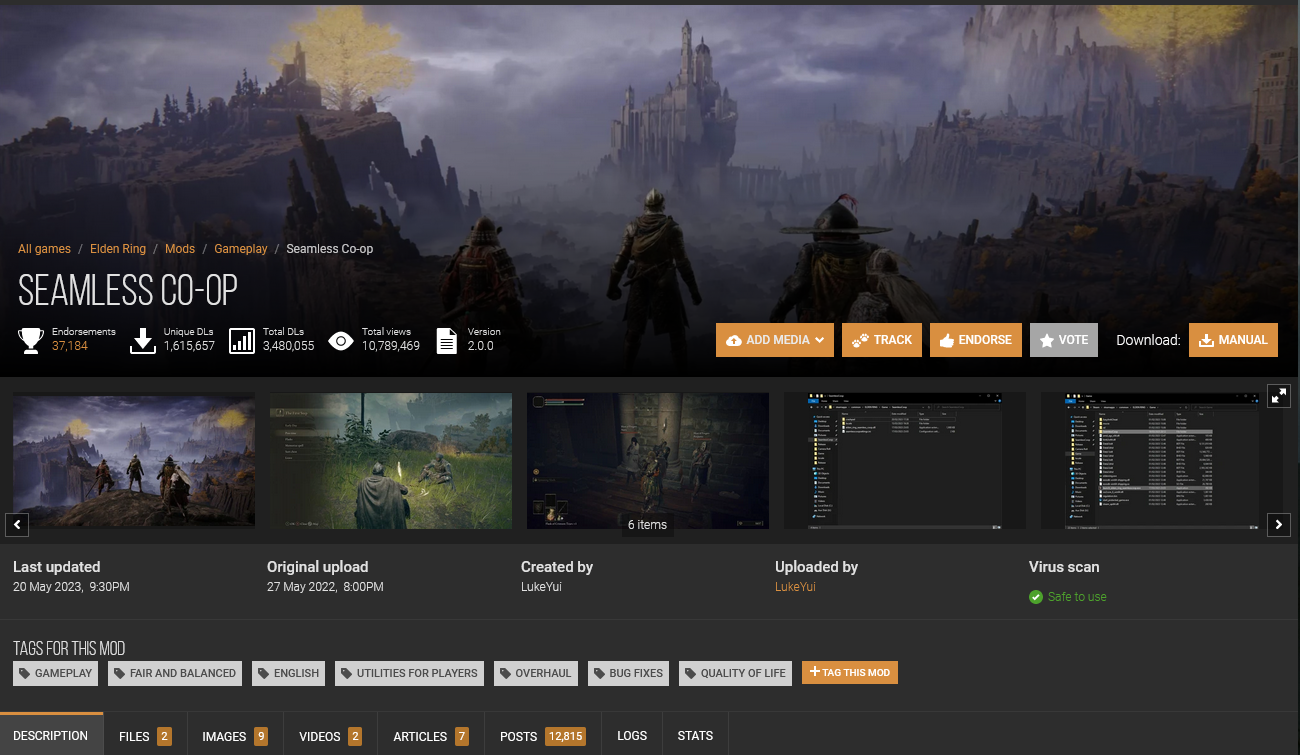
\includegraphics[scale=0.3]{images/seamless.png}
			% \caption{Mod}
		\end{figure}
	}
	\only<2>{
		\begin{figure}
			\centering
			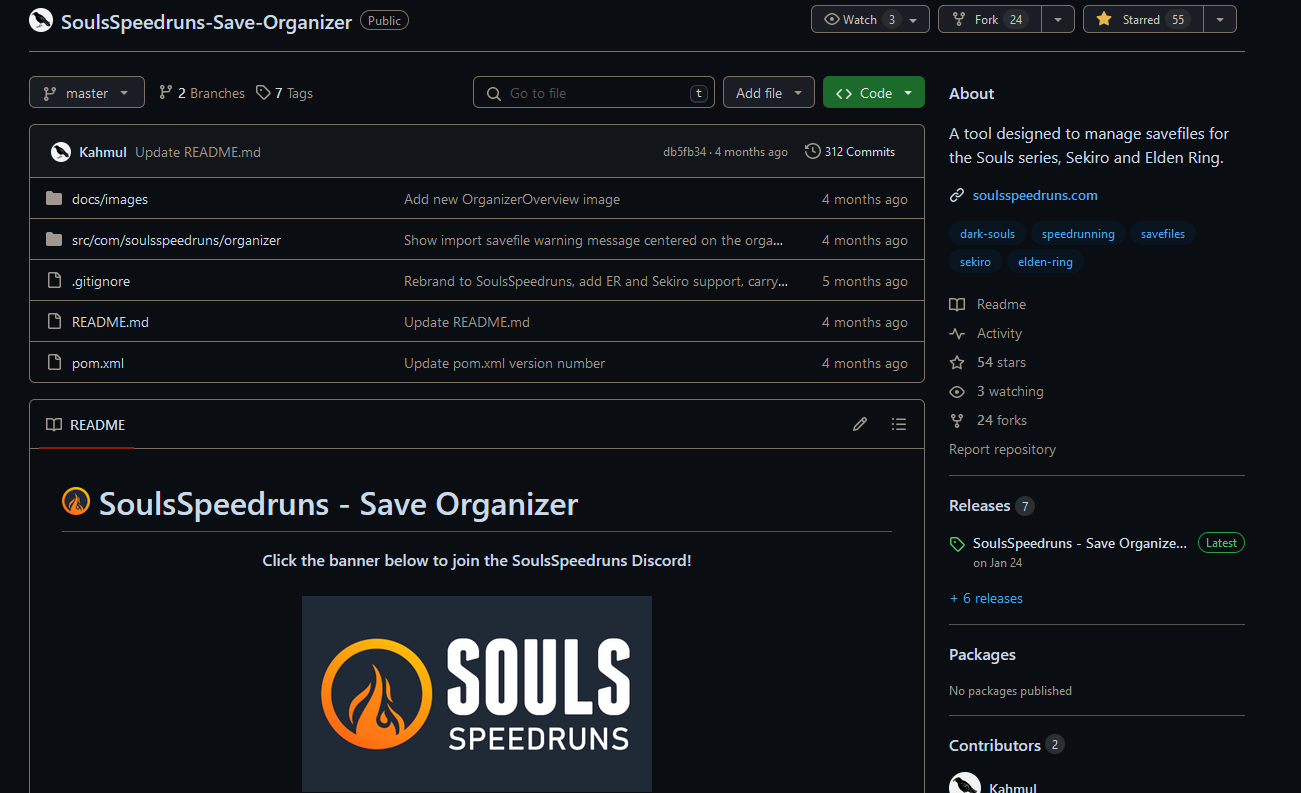
\includegraphics[scale=0.3]{images/speedsouls.png}
			% \caption{Save Manager}
		\end{figure}
	}
	\only<3>{
		\begin{figure}
			\centering
			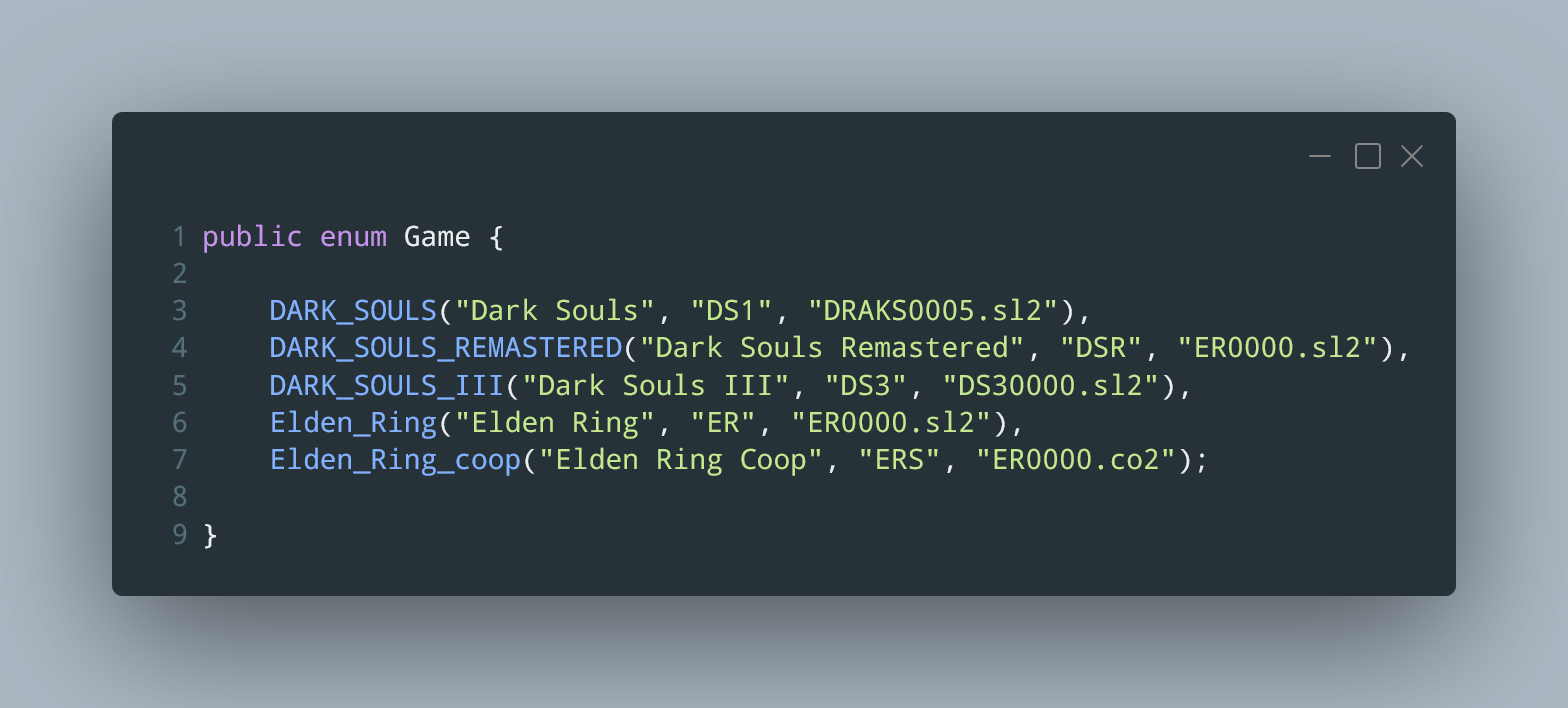
\includegraphics[scale=0.25]{images/carbon.png}
			% \caption{Code}
		\end{figure}
	}

\end{frame}
\section{Was macht die Linux Foundation?}

\begin{frame}{Was macht die Linux Foundation?}
	\begin{itemize}
		\item<1-> Mit eigenen Worten:\say{Empowering generations of open source innovators.}\cite{About}
		\item<2-> Open Source Projekte unterstützen
		\item<3-> Für offene Standarts Einsetzen
		\item <4->Entwicklung von Linux unterstützen
		\item<5-> Events Organisieren\cite{Events}
		\item<6-> Entwickler ausbilden\cite{Training}
	\end{itemize}

\end{frame}

\begin{frame}{Wie macht sie das?}
	\begin{itemize}
		\item <1->\say{Foundation as a Service}\cite{Grundprinziepe}
		\item <2->Finanzielle Unterstützung
		\item <3->Rechtlicher Schutz
		\item <4->Lernmaterialien und Zertifizierungen anbieten\cite{Training}
	\end{itemize}
\end{frame}
\begin{frame}{Wo macht sie das?}
	\begin{itemize}
		\item Weltweit mit Sitzen in:
		      \begin{itemize}
			      \item Hauptsitz in San Francisco \cite{Locations}
			      \item Sitz in Japan\cite{Locations}
			      \item Sitz in Belgien\cite{Locations}
		      \end{itemize}
	\end{itemize}
\end{frame}
\begin{frame}{Gesuchte Stellen} \begin{itemize}

		\item	Hauptsächlich Managment Positionen
	\end{itemize}
	\begin{figure}
		\centering
		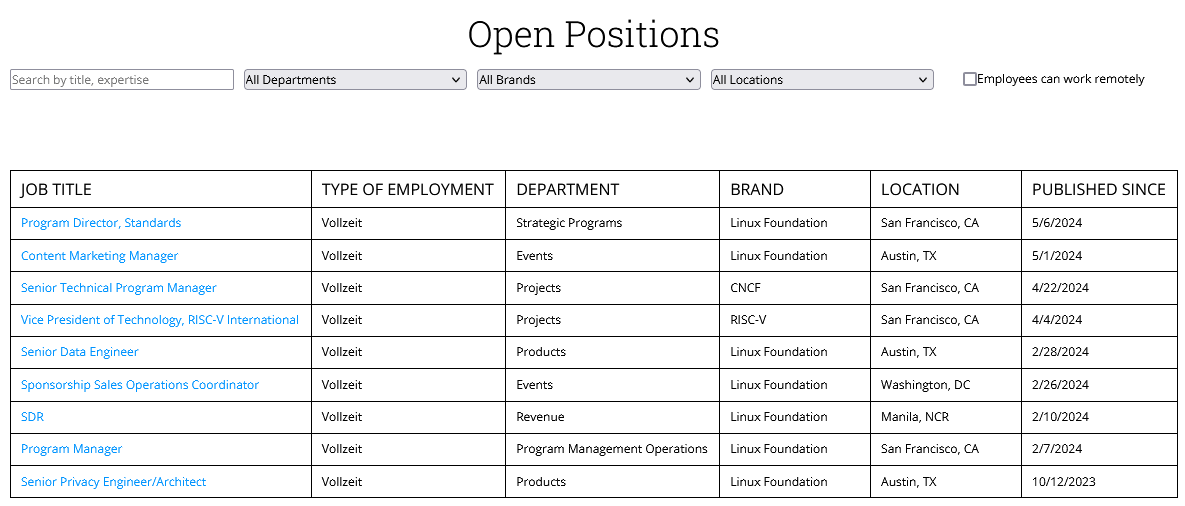
\includegraphics[scale=0.4]{images/jobs.png}\cite{Positionen}
		% \caption{Offene Stellen}
	\end{figure}

\end{frame}
\section {Ziele der Firma}
\subsection {Haupt und Nebenziele}
\begin{frame}{Hauptziele und Nebenziele}
	\begin{itemize}
		\item <1-> Hauptziele
		      \begin{itemize}
			      \item<2->Offenheit in Software zu fördern\cite{Grundprinziepe}
		      \end{itemize}
	\end{itemize}
	\begin{itemize}
		\item <3-> Nebenziele
		      \begin{itemize}
			      \item<4->Geld auftreiben
		      \end{itemize}
	\end{itemize}
\end{frame}

\subsection {komplementäre und konkurierende Ziele}
\begin{frame}{komplementäre und konkurierende Ziele}
	\begin{itemize}
		\item komplementär
		      \begin{itemize}
			      \item Open Source Community Unterstützen, Events Hosten und Entwickler ausbilden
		      \end{itemize}
	\end{itemize}
	\begin{itemize}
		\item konkurierend
		      \begin{itemize}
			      \item Durch Einhaltung der Grundprinzipien weniger Möglichkeiten an Kapital zu kommen
		      \end{itemize}
	\end{itemize}
\end{frame}
\begin{frame}{lang/kurzfristige Ziele}
	\begin{itemize}
		\item langfristig
		      \begin{itemize}
			      \item Offenheit in der nächsten Entwicklergeneration fördern
		      \end{itemize}
	\end{itemize}
	\begin{itemize}
		\item kurzfristig
		      \begin{itemize}
			      \item Neue Sponsoren finden
		      \end{itemize}
	\end{itemize}
\end{frame}

\section{Quellen}
\begin{frame}{Quellen}
	\centering
	\url{https://github.com/Stefanistkuhl/obsidianschule/blob/main/2.Klasse/Ipt/dummeididreckspr\%C3\%A4si/quellen.bib}
	\bibliographystyle{plain}
	\bibliography{./quellen.bib}
\end{frame}
\begin{frame}{Danke für eure Aufmerksamkeit!}
\end{frame}

\end{document}
